\documentclass[12pt,tikz]{standalone}

\usepackage{graphicx}
\usetikzlibrary{positioning}
\begin{document}

\newcommand{\state}[2]{%
  $s = $ \texttt{#1}\\
  $p = $ \texttt{#2}
}

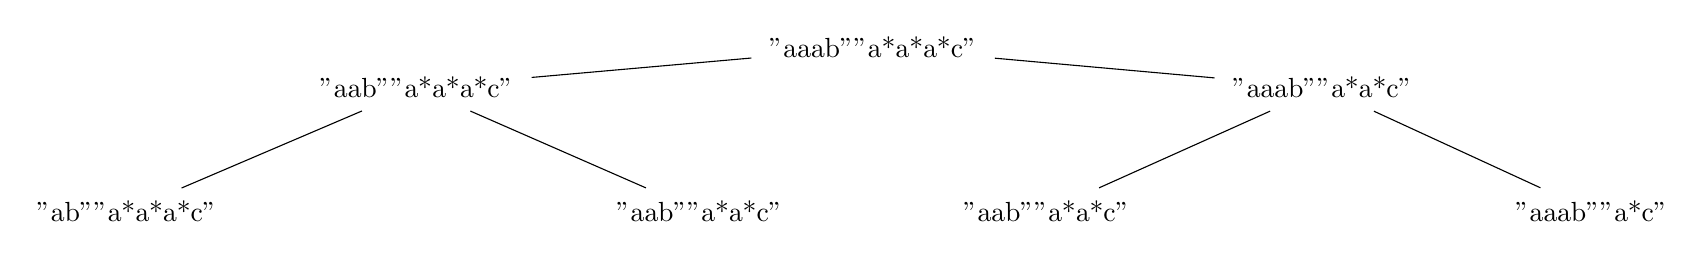
\begin{tikzpicture}[align=center, draw, black, shorten >=3pt, shorten <=3pt, node distance = 1.5cm]
  \node (root) {\state{"aaab"}{"a*a*a*c"}};
  \node[below left = 0cm and 3cm of root] (L) {\state{"aab"}{"a*a*a*c"}};
  \draw (root) -- (L);
  \node[below left = of L] (LL) {\state{"ab"}{"a*a*a*c"}};
  \draw (L) -- (LL);
  \node[below right = of L] (LR) {\state{"aab"}{"a*a*c"}};
  \draw (L) -- (LR);

  \node[below right = 0cm and 3cm of root] (R) {\state{"aaab"}{"a*a*c"}};
  \draw (root) -- (R);
  \node[below left = of R] (RL) {\state{"aab"}{"a*a*c"}};
  \draw (R) -- (RL);
  \node[below right = of R] (RR) {\state{"aaab"}{"a*c"}};
  \draw (R) -- (RR);
\end{tikzpicture}
\end{document}

